\documentclass[a4paper]{report}
\usepackage{mathtools}
\usepackage{graphicx}
\usepackage{verbatim} 
\scrollmode
%
\usepackage{amsmath}
\usepackage{amsfonts}
\usepackage{amssymb}
\usepackage{latexsym}
\usepackage{stmaryrd}
\usepackage{array}
\usepackage{exscale}

\usepackage[driverfallback=hypertex]{hyperref}

%\graphicspath{ {"C:/Users/l_joh/Desktop/tree.jpg"} }

\setcounter{secnumdepth}{2}
\setcounter{tocdepth}{1}

\begin{document}

\title{Reductions for NP-complete problems}

\author{Luke Bevan John\\
  Computer Science Department\\
  Swansea University\\
  Swansea, SA1 8EN, UK
}
\date{}

\maketitle

\begin{abstract}
  Investigation into reductions from SAT to $N$-Queens completion.
\end{abstract}

\tableofcontents


\setcounter{chapter}{-1}

\chapter{TODOS etc.}
\label{cha:todos}

\section{On Latex}
\label{sec:todoslatex}

\cite{lamport94}


\section{Todos}
\label{sec:todostodos}

\begin{enumerate}
\item Consolidate Git-repositories.
\item Next meeting: looking at the C++ code.
  \begin{enumerate}
  \item Testing.
  \item Documentation.
  \item Possibly a Solver
  \end{enumerate}
\item Research: improving the reduction SAT to 3SAT:
  \begin{enumerate}
  \item Examples (complete) and Written out.
  \item Initial concepts.
  \item Literature overview.
  \item literature search about the topic of reductions SAT --> 3-SAT.
  \item for every relevant piece of literature found, write one paragraph, what's in that peice about relevant to our topic.
  \end{enumerate}
\item Oliver Email\\
 just to summarise the discussion we had:
  \begin{enumerate}
     \item We will focus on the reductions, their implementations and experimental evaluation.
    \item With the implementations, C++ will be learned.
    \item The experimental evaluation can be extended to include the use the machine-learning tools for automatic configuration of the reductions.
    \item start providing basic definitions. \\ 
\\ Oliver
  \end{enumerate}
\end{enumerate}

\section{Plan}
\label{sec:Plan}
\begin{enumerate}
\item add karp paper to bibtex document.\cite{Karp1972NP}
\item write paragraph on paper.

\end{enumerate}



\chapter {Introduction}
\label{cha:Introduction}

\section{Background}
\label{sec:Background}



\chapter{SAT to 3SAT}
\label{cha:sat13}

\begin{enumerate}
\item \cite{Cook1971NP}
  \begin{enumerate}
  \item Theorem proves that every language in co-NP can be reduced to TAUT.
  \item The proof of Theorem 1 actually shows that SAT (for CNF) is NP-complete.
  \item Theorem 2 shows that 3-CNF (every clause has length at most 3) is NP-complete. This happens by splitting up a clause $x_1 \vee \dots \vee x_s$ into
    \begin{displaymath}
      v \vee x_1 \vee x_2, \quad \neg v \vee x_3 \vee \dots \vee x_s.
    \end{displaymath}
XXX proof of correctness YOURSELF

a couple of sentences WHAT is to be proven

Proof of correctness : proof that the alogorithm when provided an input produces the expected (and correct) output.\\

Question : Prove, assuming SAT is NP-complete, that a reduction from CNF SAT to 3-CNF, is evidence that 3-CNF is also NP-complete.\\

a couple of sentences for the arguments
\\
F is CNF SAT formula.\\ 
$F =  C = \bigwedge_{j=1}^{n} c_j = c_1 \wedge c_2 \wedge \dots \wedge c_n$
%$c = x_1 \vee x_2 \vee \dots \vee x_s$

%$n =$ total number of clause in clause set
C is a clause set.
$c \in C$.\\
$c_i = X_i = \bigvee_{j=1}^{s} x_{ij} =  (x_{i1} \vee x_{i2} \vee \dots \vee x_{is})$\\
$s > 3 $\\
$x_{ij}$ is an atom or negation of an atom.
$x \in X$.\\
\\
\\
F$'$ is a CNF 3-SAT formular.\\
$F' =  C' = \bigwedge_{j=1}^{n} c'_j = c_1 \wedge c_2 \wedge \dots \wedge c_n$\\
$C'$ is a clause set.
$c' \in C' \quad c'$ is a clause with only three atoms.\\
$c'_i = X_i \cup X'_i = \bigvee_{j=1}^{s'} x_{ij} \bigvee_{k=1}^{s'-3}v_{ik}= \\= (x_{i1} \wedge x_{i2} \wedge \dots \wedge x_{is'}) \vee (v_{ik} \wedge \neg v_{ik})
\\ =  (x_{i1} \vee x_{i2} \vee v_{ik}) \wedge  (\neg v_{ik} \vee x_{i3} \vee  v_{i(k+1)}) \wedge \dots \wedge   (\neg v_{i(s'-3)} \vee x_{i(s'-1)} \vee x_{is'})$\\
$s' \subseteq s > 3  $\\
$x_{ij}$ is an atom or negation of an atom. $v_{ik}$ is a new atom .\\
$x \in X$.$v \in X'$.\\
\\
$F'$ is only satsifiable iff $F$ is satisfiable, also $c'_i$ is equivalent to $c_i$ as the compound proposition $(v_{ik} \wedge \neg v_{ik})$ is a contradiction and according to identity laws effectivly leaves the original clause's unchnaged, just as in addition, adding a $(1 + -1)$ to an eqaution results in the same equation. 
\\

  \item This all in a different language.
  \end{enumerate}

\end{enumerate}
\begin{comment}
$\phi$ = $( x_1 \wedge x_2 ) \vee (\neg x_1 \vee x_3) \wedge \neg x_2$ 
\\
\\
\\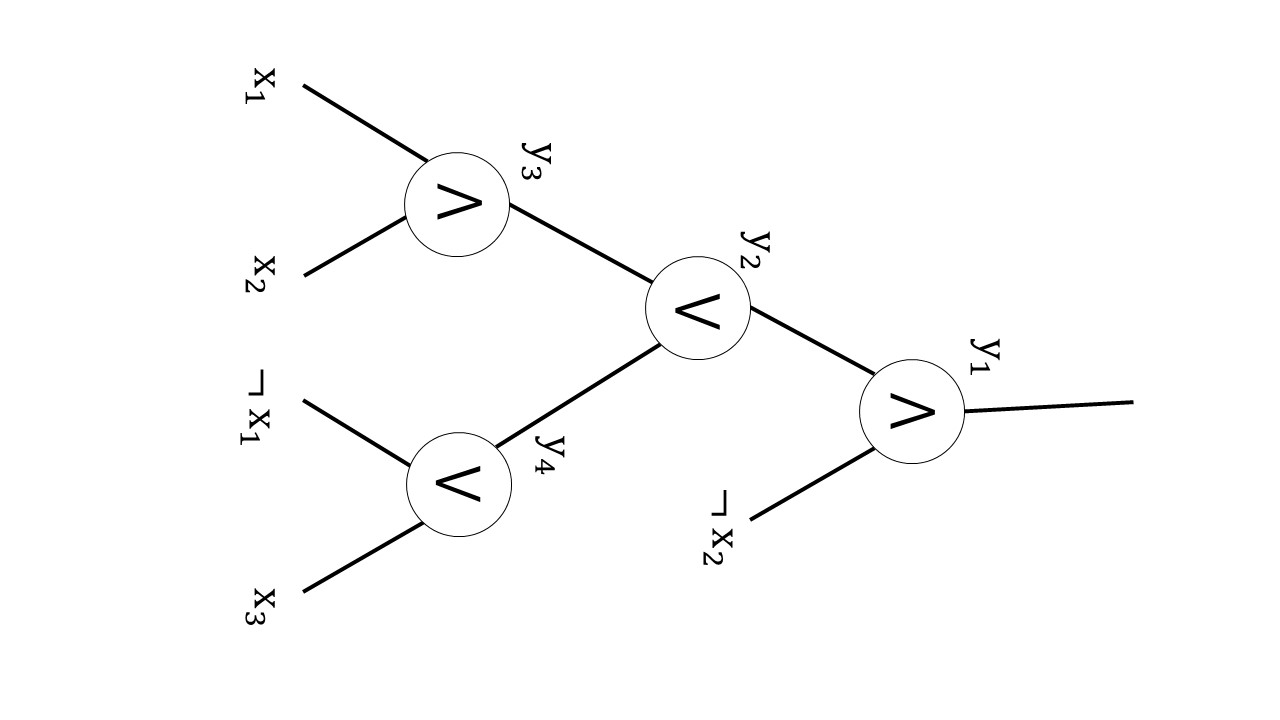
\includegraphics[scale = 0.3 , angle = 90]{tree.jpg}\\
$\phi ' $
\begin{tabular}{|c|}
\hline
$ = y_1 \wedge$ $(y_1$  $\iff$ $( y_2 \wedge \neg x_2))$   \\
$(y_2$  $\iff$ $( y_3 \vee  y_4))$   \\
$(y_3$  $\iff$ $( x_1 \wedge  x_2))$   \\
$(y_4$  $\iff$ $( \neg x_1 \vee  x_3))$   \\
\hline
\end{tabular}\\
\\
\\%$p \iff q \equiv (p \wedge q) \vee ( \neg p \wedge \neg q)$
\\ 
truth table for biconditional statment\quad$ p \iff q $\\
\begin{tabular}{|c|c|c|}
\hline
p & q&  \\
\hline
T & T & T \\
T&F&F\\
F&T&F\\
F&F&T\\
\hline
\end{tabular}\\
\\
\\
\begin{tabular}{ |c|c|c|c|c| }
\hline
p&
\multicolumn{2}{|c|} {q}\\
\hline
$y_1$&$y_2$&$\neg y_2$&Clause 1\\
\hline		
1&1&0&	FALSE*\\
1&1&1&	TRUE\\
1&0&0& 	FALSE*\\
1&0&1&	FALSE*\\
0&1&0&	TRUE\\
0&1&1&        FALSE*\\
0&0&0&	TRUE\\
0&0&1&	TRUE\\
\hline
\end{tabular}\\
$\neg C_1 = (y_1 \wedge y_2 \wedge x_2) \vee (y_1 \wedge \neg y_2 \wedge x_2) \vee (y_1 \wedge \neg y_2 \wedge \neg x_2) \vee (\neg y_1 \wedge y_2 \wedge \neg x_2)$\\
\\
\begin{tabular}{|c|}
\hline
Demorgans Law\\
$\neg( p \wedge q ) = \neg p \vee \neg q$\\
$\neg( p \vee q ) = \neg p \wedge \neg q$\\
\hline
\end{tabular}\\
\\
$CNF\quad C_1 = (\neg y_1 \vee \neg y_2 \vee \neg x_2) \wedge ( \neg y_1 \vee y_2 \vee \neg x_2) \wedge (\neg y_1 \vee y_2 \vee x_2) \wedge ( y_1 \vee \neg y_2 \vee x_2) $\\
\\
\\
\begin{tabular}{ |c|c|c|c|c| }
\hline
$y_2$&$y_3$&$y_4$&Clause 2\\
\hline		
1&1&0&	TRUE\\
1&1&1&	TRUE\\
1&0&0&	FALSE*\\
1&0&1&	TRUE\\
0&1&0&	FALSE*\\
0&1&1&	FALSE*\\
0&0&0&	TRUE\\
0&0&1&	FALSE*\\
\hline
\end{tabular}\\
\end{comment}


\section{3SAT to 1-in-3-SAT}
\label{sec:3satto13}



\bibliographystyle{plainurl}
\bibliography{Bibliography}

\end{document}